\chapter{MARCO TE�RICO}
%\chapter{Introducci�n}
%\chaptermark{version for header}
\markboth{Introducci�n}{}
Es una arquitectura de \gls{sig:BI} dirigido a informes interactivos y datos explorables de m�ltiples fuentes. De acuerdo con Gartner,  la firma de investigaci�n y asesoramiento de la tecnolog�a de la informaci�n en Am�rica, data discovery se ha convertido en una arquitectura dominante en 2012.

Jill Dyche llama data discovery ?descubrimiento del conocimiento? y la define como "la detecci�n de patrones en los datos?. Estos patrones son muy espec�ficos y aparentemente arbitrarios para especificar, y el analista estar�a jugando un juego de adivinanzas tratando de descifrar todos los posibles patrones en la base de datos. En cambio, las herramientas especiales de software para data discovery encuentra los patrones y dicen al analista lo que y donde encontrarlos.

El actual vicepresidente(2013-2014) de buenas pr�cticas en SAS Institute dice que no es de extra�ar que la definici�n de data discovery se asemeja a la definici�n de miner�a de datos:

"La miner�a de datos un subcampo interdisciplinario de ciencias de la computaci�n, es el proceso computacional de descubrir patrones en grandes conjuntos de datos involucrando m�todos de la  inteligencia artificial, aprendizaje autom�tico, estad�stica y sistemas de bases de datos. El objetivo general del proceso de miner�a de datos es extraer informaci�n de un conjunto de datos y transformarla en una estructura comprensible para su uso posterior. Aparte de la etapa de an�lisis en bruto, trata de bases de datos y gesti�n de datos, preprocesamiento de datos, consideraciones de modelo e inferencia, m�tricas interesantes, consideraciones de complejidad, postprocesado de las estructuras descubiertas, visualizaci�n y actualizaci�n en l�nea ".

Tambi�n puede ser referido como Business Discovery.
\section{Objetivos}
Escribir sobre los objetivos
Como puede ser visto en la figura \ref{fig:BI}.

\begin{figure}[!htb]
	\centering
	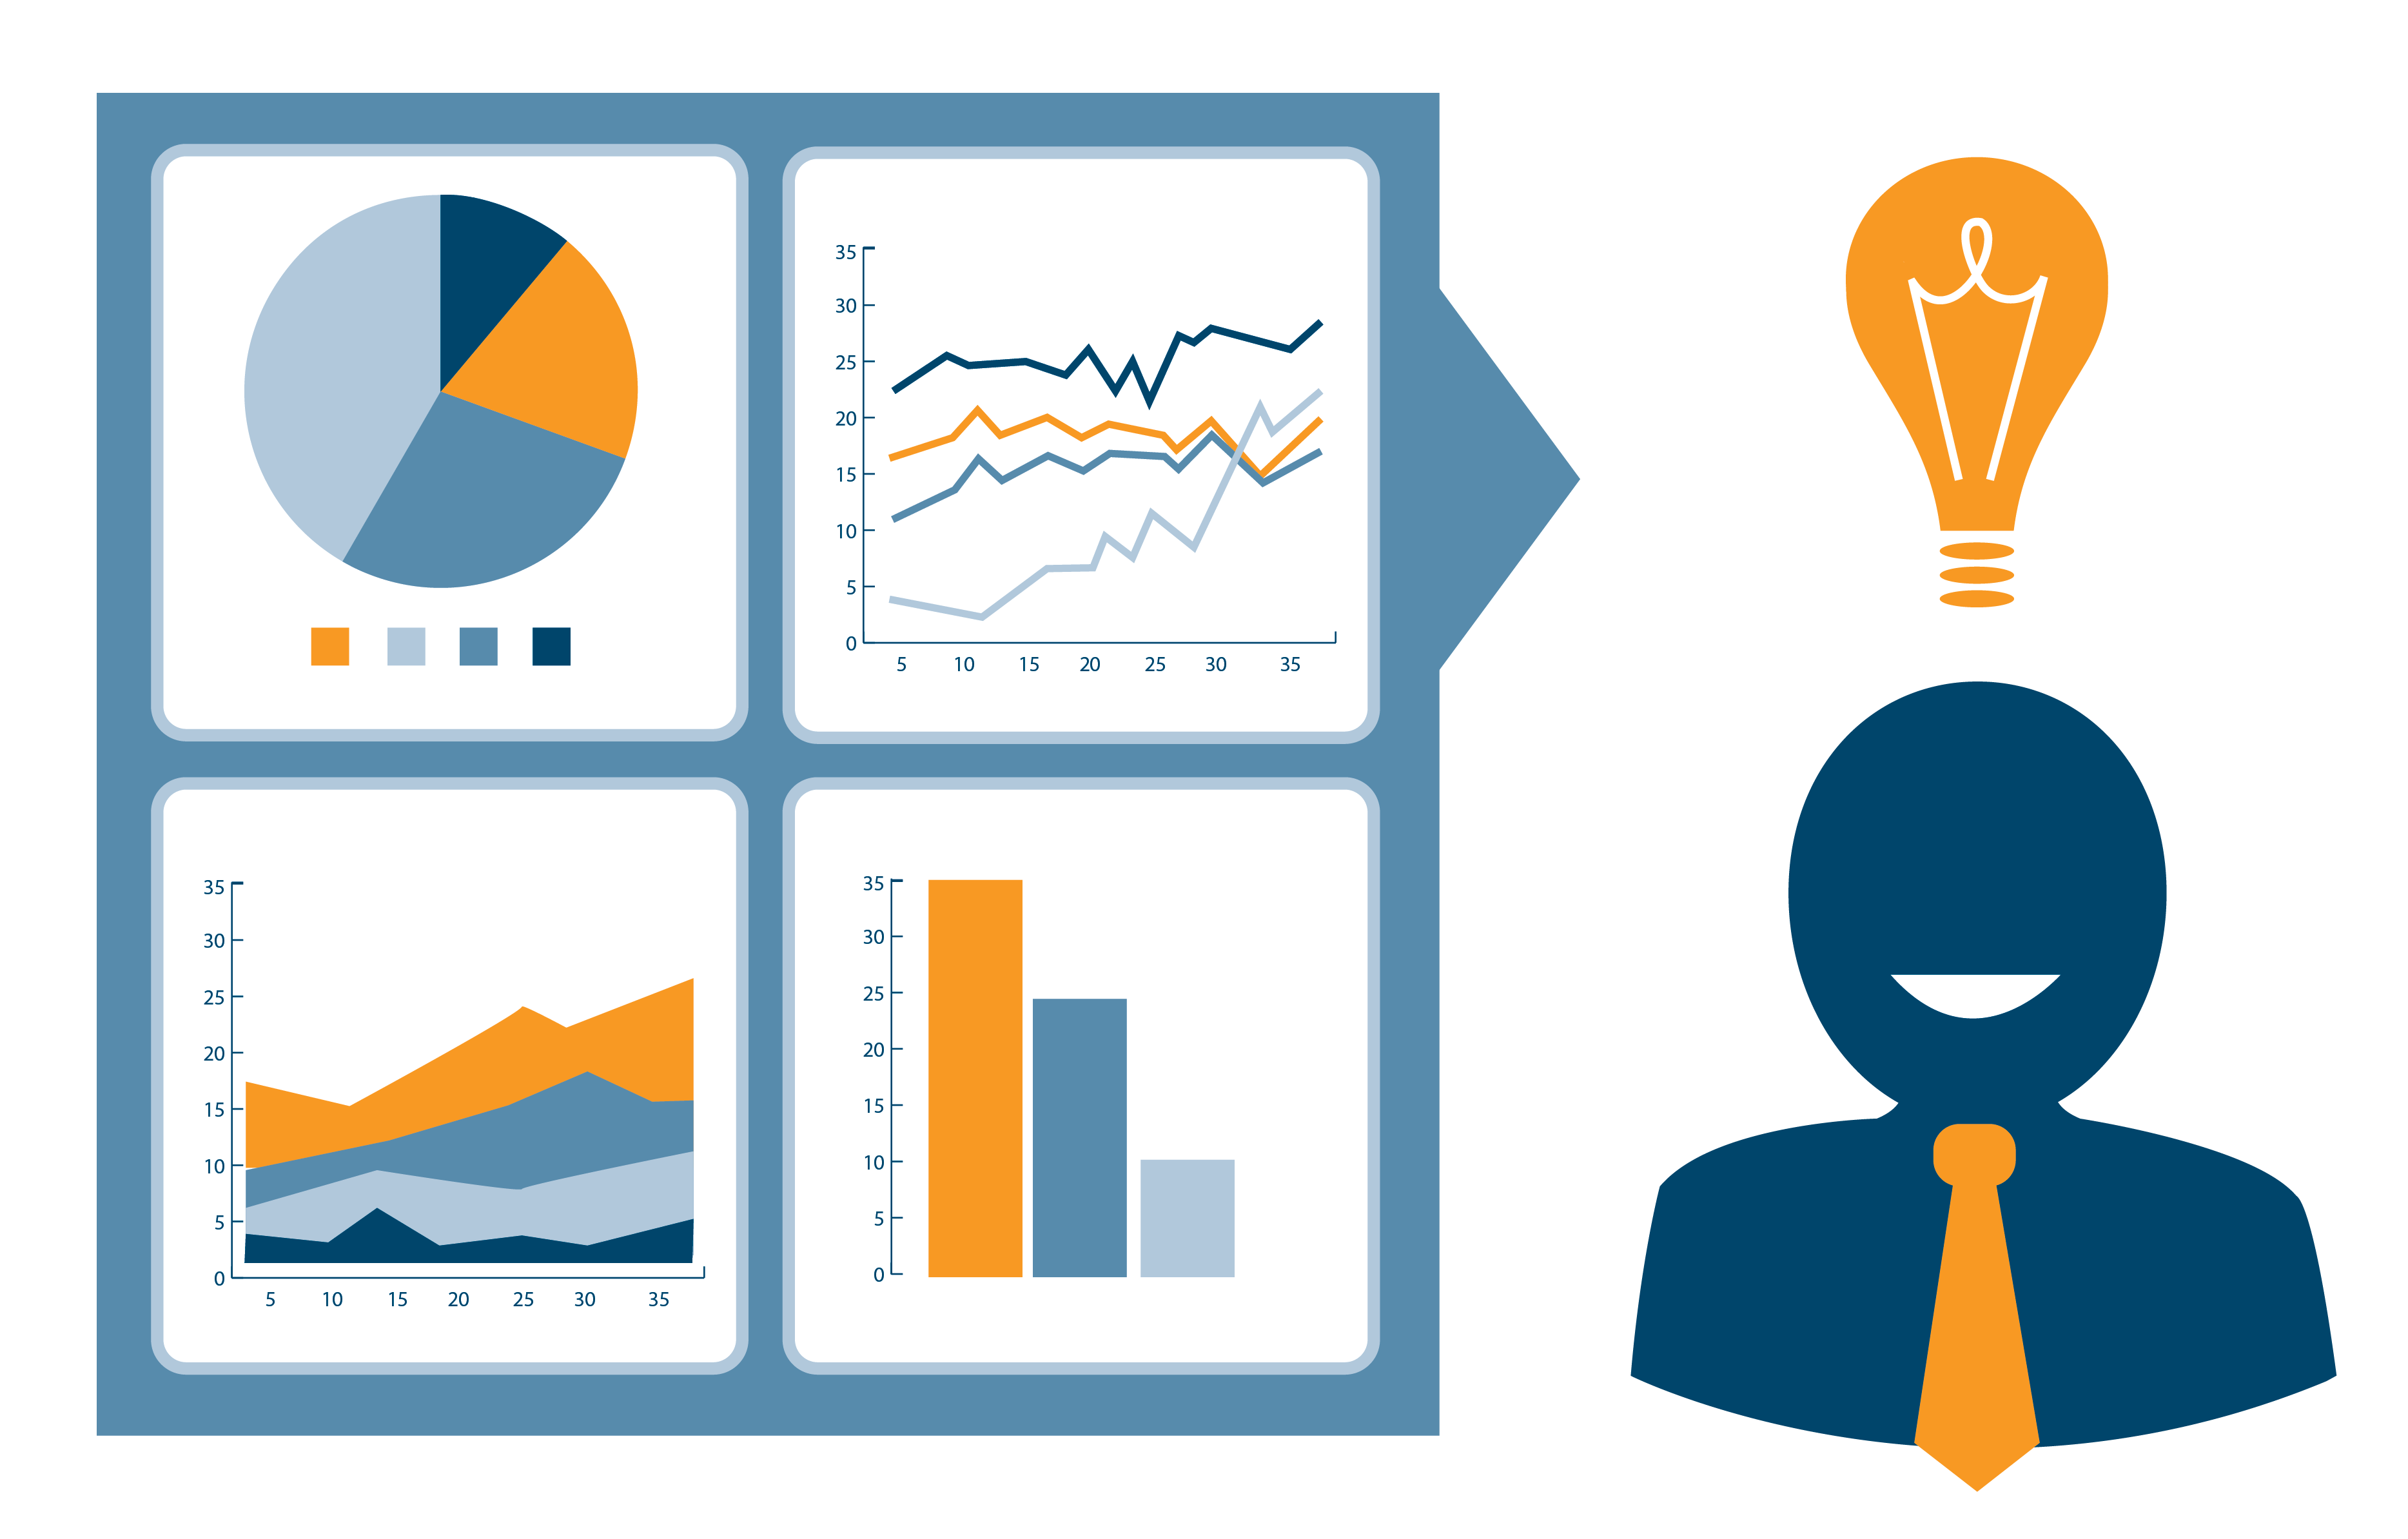
\includegraphics[width=150mm]{insight-bi.png}
	\caption{Representaci�n de un dashboard \gls{sig:BI}}
	\label{fig:BI}
	\cite{kumari2013business}
\end{figure}
\subsection{Sub-Secci�n Ejemplo}
Un ejemplo nomas

\section[dlsadk]{Business Intelligence}
Business Intelligence (from reference \cite{kumari2013business})

